\subsection{Analyse von den Resultaten der «Fussabdrücke»}
Der Fragebogen von WWF zeigt auf wie viele Planeten man bräuchte,  wenn alle Menschen denselben
Lebensstil hätten, wie derjenige der diesen Fragebogen ausfüllt. Bei unserer Gruppe lagen die Werte
zwischen 2,2 und 2,9. Der Durchschnitt liegt bei 2,575. Dies bedeutet, dass unser durchschnittlicher Lebensstil ungefähr 2,5 Erden bräuchte.

Interessant zu sehen ist, dass alle Mitglieder genau gleich viel Energie verbrauchen in den
öffentlichen Diensten. Dies entspricht nur wenig mehr als dem Idealwert, bei welchem wir nur eine
Erde brauchen. Bei der Mobilität, Konsum, Wohnen und Ernährung liegen alle Mitglieder unserer Gruppe
im x-fachen Bereich über dem Idealwert. Hier besteht das grösste Verbesserungspotenzial. Bei der
Mobilität kann man unter anderem auf einen Auslandflug verzichten. Denn eine Stunde im Flugzeug entspricht circa einem Monat Autofahren. 

Auch bei der Ernährung kann man sich einfach verbessern. Man sollte versuchen vor allem regionale
Produkte zu konsumieren. Ebenfalls ist Fleisch verzehren eine grosse Belastung für die Umwelt, dies
kann jedoch simpel reduziert werden in dem man den Verzehr reduziert oder gar ganz weglässt. Was uns
in der Gruppe generell erstaunt hat ist die Tatsache,  dass Eier und Milchprodukte die Umwelt ebenfalls sehr belasten. 

Etwas mehr Aufwand bedarf die Energieeinsparung im Bereich Wohnen. Eine radikale aber sehr gute
Option ist es das Auswechseln der Ölheizung mit beispielsweise einer Pelletheizung, welche einiges
umweltfreundlicher ist. 
Es lassen sich aber auch schon mit kleineren Aufwand Verbesserungen erzielen. So sollte man bei
Elektrogeräten darauf achten, dass sie mit einer guten Energieklasse bewertet wurden.
 
Als Abschluss kann man sagen, dass unsere Gruppe zwar klar unter dem schweizerischen Durchschnitt
liegt aber dennoch einiges machen kann, um die Belastung an der Umwelt zu verringern. 

\subsection{Einkaufsverhalten}

Zur Untersuchung des Konsumverhaltens wurden vorgängig unabhängig von der Gruppe Daten erfasst.
Dabei wurde über eine Woche untersucht, wo die Lebensmittel genau bezogen wurden. Durch das
Analysieren der Daten resultierte die Grafik. Daraus ist klar ersichtlich, dass der Grossteil der Produkte von Grosshändler wie Migros und Coop bezogen werden.
 \begin{figure}[H]
	\centering
	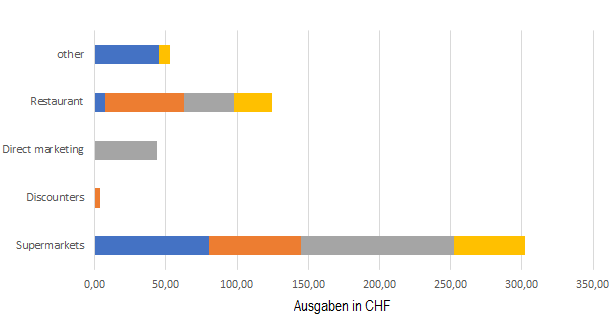
\includegraphics[width=0.9\textwidth]{ta}
	\caption{Analyse des Einkaufverhalten der einzelnen Studierenden}
\end{figure}

Diskussionen in der Gruppe haben ergeben, dass die Hauptgründe dafür vor allem die Verfügbarkeit und
die grosse Auswahl sind. Dabei stellte sich heraus, dass sowohl Migros wie auch Coop mittlerweile
sehr viele regionale und nachhaltige Produkte im Sortiment haben. Somit ist  das Streben nach
Nachhaltigkeit nicht von der Frage, wo wir einkaufen, sondern was wir einkaufen abhängig.
